\documentclass[a4paper,11pt]{article}
\usepackage[utf8]{inputenc}
\usepackage[czech]{babel}
\usepackage[T1]{fontenc}
\usepackage{amsmath}
\usepackage{amsfonts}
\usepackage{amssymb}
\usepackage{graphicx}
\usepackage{mathtools}
\usepackage{fancyhdr}
\usepackage{epstopdf}
\usepackage[hidelinks]{hyperref}
\usepackage{float}
\usepackage{gensymb}
\usepackage[final]{pdfpages}
\usepackage{a4wide}
\renewcommand{\arraystretch}{1.5}
%\renewcommand{\baselinestretch}{1.25}

\title{Automatické řízení \\
	Semestrální práce}
\usepackage[top=25mm, left=35mm, right=25mm, bottom=25mm]{geometry}
\author{Miroslav Bulka, Jan Cibulka}
\date{\today}	
\setlength{\parskip}{10pt}
\begin{document}
\maketitle

\begin{figure}[h]
	\centering
	
\includegraphics[width=9cm]{obrazky/fav.png}
\end{figure}
\clearpage
\newpage


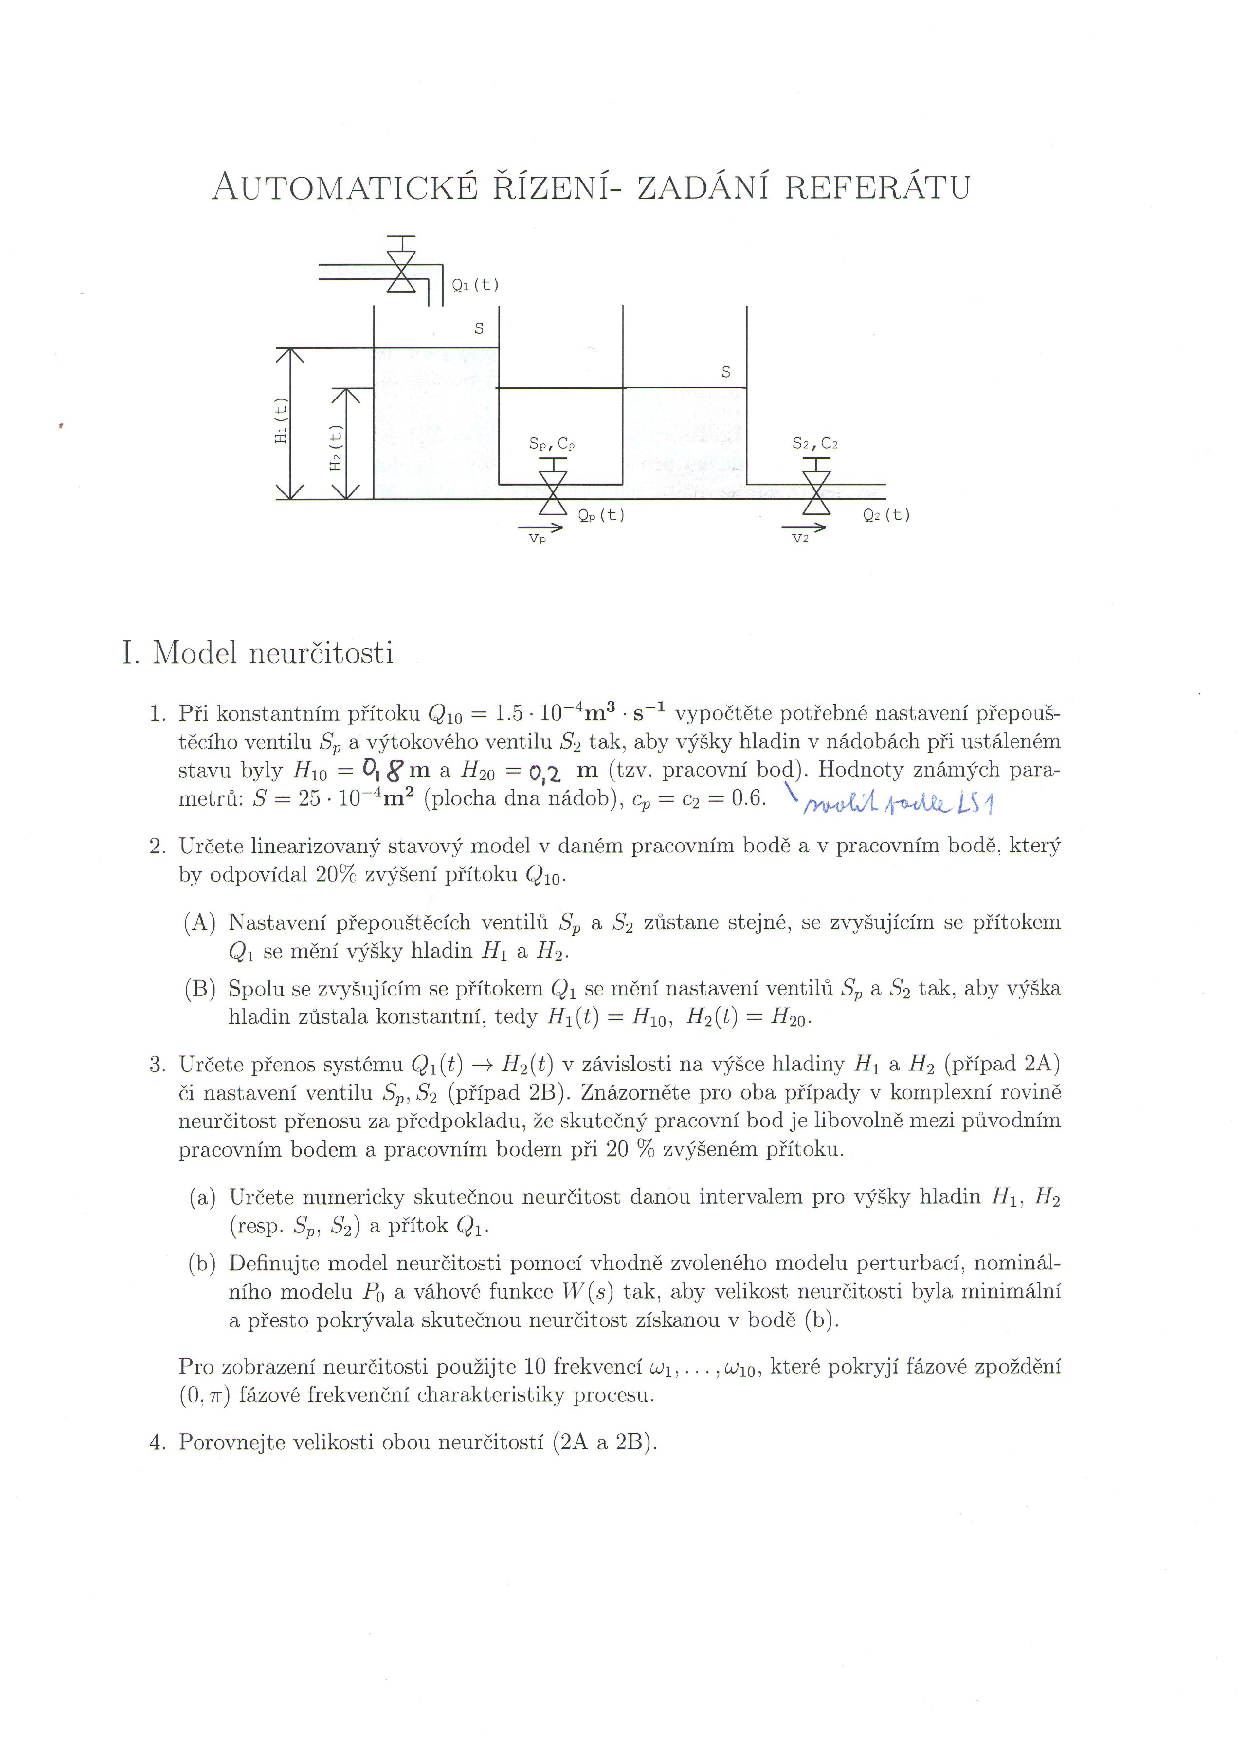
\includepdf{obrazky/Zadani1.pdf}
\newpage
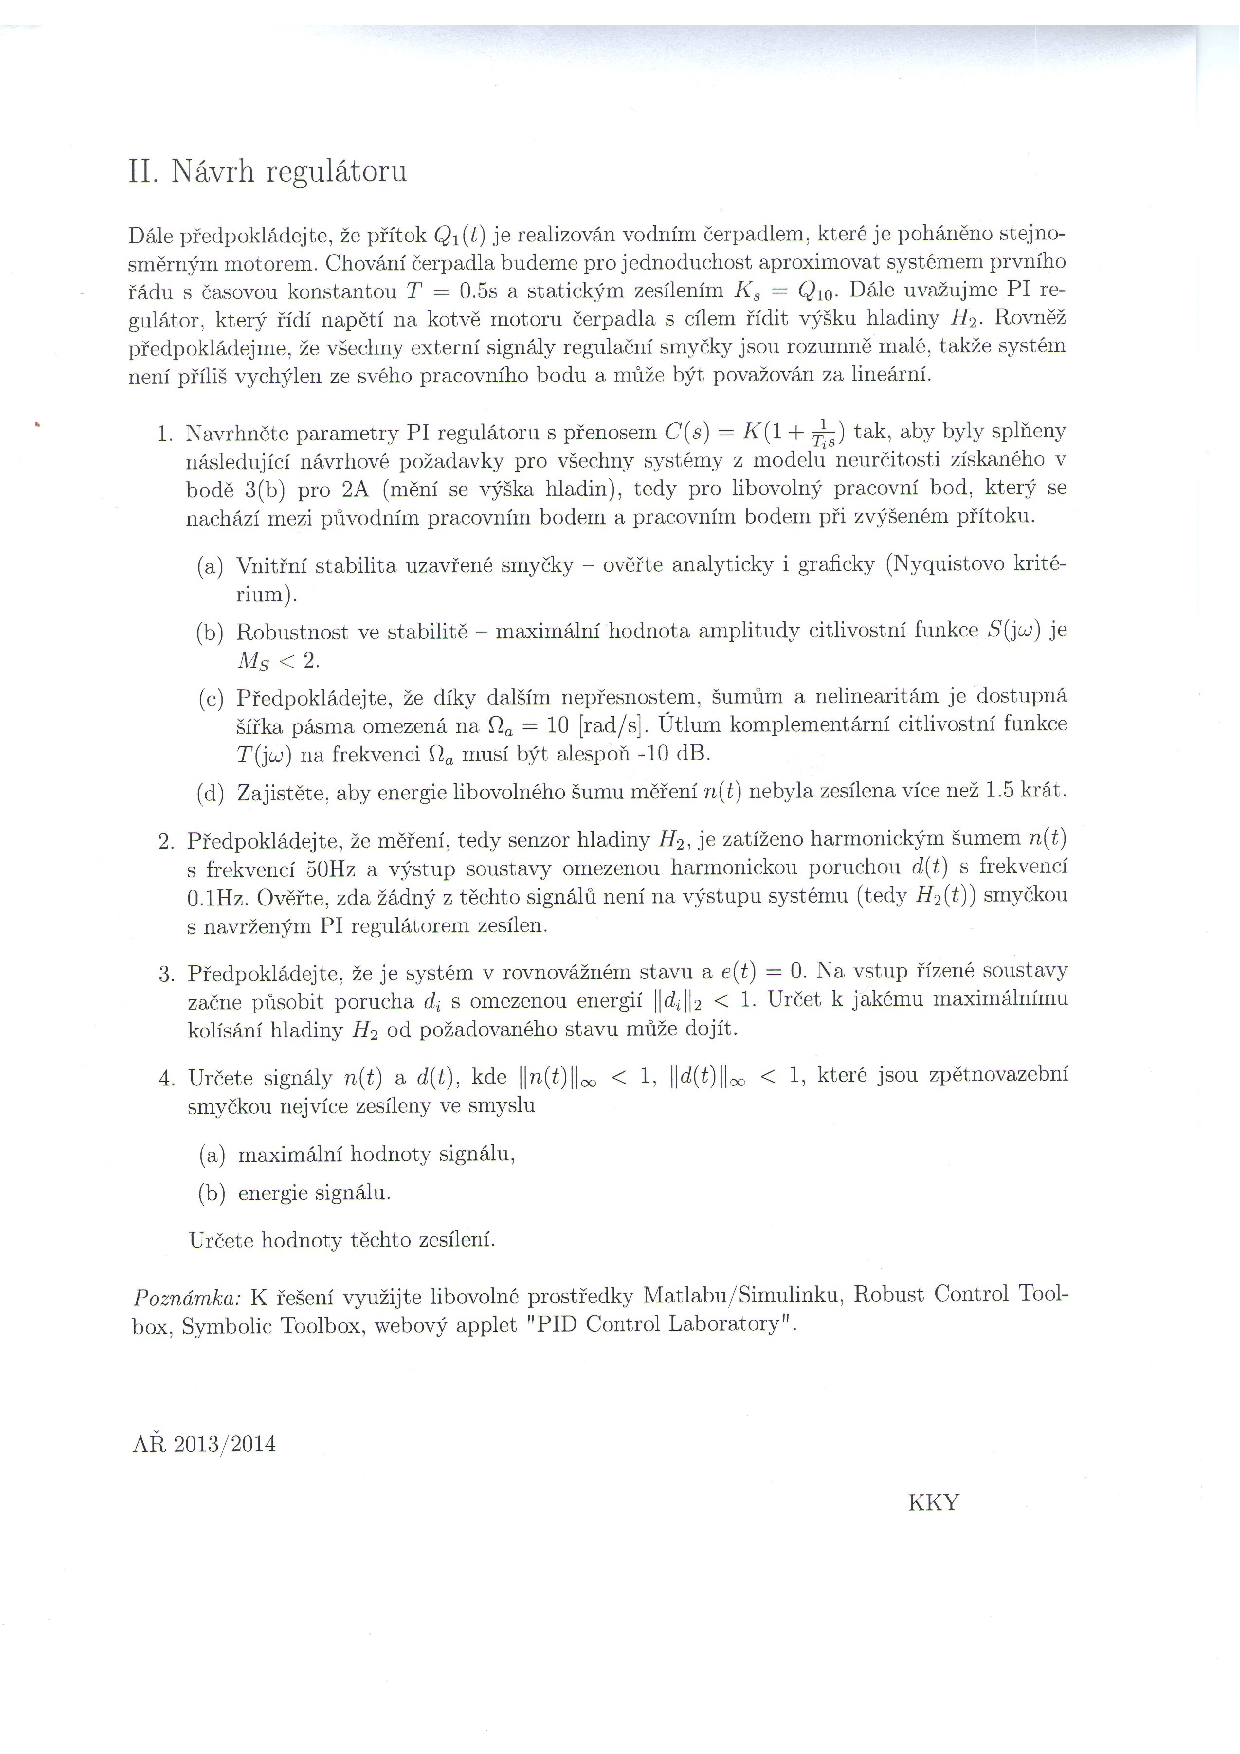
\includepdf{obrazky/Zadani2.pdf}
\newpage

\tableofcontents
\newpage
\section{Řešení - Model neurčitosti}
\subsection{První úkol - výpočet nastavení ventilů}
Máme konstantní přítok $Q_{1}=Q_{10}=1.5\cdot 10^{-4}m^{3}s^{-1}$, přičemž víme, že:
\begin{equation}
\left [\begin{array}{cc}
\frac{dV_{1}}{dt}\\
\frac{dV_{2}}{dt}
\end{array}\right ] = 
\left [\begin{array}{cc}
Q_{1}-Q_{p}\\
Q_{p}-Q_{2}\end{array}\right ] = 
\left [\begin{array}{cc}
Q_{1}-c_{p}S_{p}v_{p}\\
c_{p}S_{p}v_{p}-c_{2}S_{2}v_{2}\end{array}\right ].
\end{equation}
Z Bernoulliho zákona pak odvodíme:
\begin{equation}
\left [\begin{array}{cc}
v_{p} \\
v_{2}
\end{array}\right ] = 
\left [\begin{array}{cc}
\sqrt{2g\cdot (H_{1}-H_{2})}\\
\sqrt{2g\cdot (H_{2})}\end{array}\right ].
\end{equation}
Daný systém popisují diferenciální rovnice:
\begin{equation}
\left [\begin{array}{cc}
\frac{dH_{1}}{dt} \\
\frac{dH_{2}}{dt}
\end{array}\right ] = 
\left [\begin{array}{cc}
\frac{1}{S}\cdot Q_{1}-\frac{S_{p}C_{p}}{S}\cdot \sqrt{2g\cdot (H_{1}-H_{2})}\\
\frac{S_{p}C_{p}}{S}\cdot \sqrt{2g\cdot \left ( H_{1}-H_{2} \right )}-\frac{S_{2}C_{2}}{S}\cdot \sqrt{2g\cdot H_{2}}\end{array}\right ].
\end{equation}
Zavedením 
$ x_{1}(t)=H_{1}(t);\;$ 
$x_{2}(t)=H_{2}(t);\;$ 
$u(t)=Q_{1}(t)\; $
získáme
\begin{equation}\label{eq:Stavove_x} 
\left [\begin{array}{cc}
\frac{dx_{1}}{dt} \\
\frac{dx_{2}}{dt}
\end{array}\right ] = 
\left [\begin{array}{cc}
\frac{1}{S}\cdot u-\frac{S_{p}C_{p}}{S}\cdot \sqrt{2g\cdot (x_{1}- x_{2})}\\
\frac{S_{p}C_{p}}{S}\cdot \sqrt{2g\cdot \left ( x_{1}-x_{2} \right )}-\frac{S_{2}C_{2}}{S}\cdot \sqrt{2g\cdot x_{2}}\end{array}\right ].
\end{equation}
Za předpokladu neměnících se hladin $H_{1}$ a $ H_{2} $ budou obě derivace nulové. Položíme je tedy nulou a díky tomu získáme požadované nastavení přepouštěcího ventilu $S_{p}$ a výtokového ventilu $S_{2}$:
\begin{equation}\label{eq:vypocet_ventilu}
\left [\begin{array}{cc}
S_{p} \\
S_{2}
\end{array}\right ] = 
\left [\begin{array}{cc}
\frac{Q_{10}}{C_{p}\cdot \sqrt{2g\left ( H_{1}-H_{2} \right )}}\\
\frac{C_{p} S_{p}\sqrt{\left ( H_{1}-H_{2} \right )}}{C_{2} \sqrt{H_{2}}}\end{array}\right ],
\end{equation}
kde po dosazení získáme:
\begin{equation}\label{eq:nastaveni_ventilu_10}
\left [\begin{array}{cc}
S_{p} \\
S_{2}
\end{array}\right ] = 
\left [\begin{array}{cc}
7.2864\cdot 10^{-5}\\
1.2620\cdot 10^{-4}\end{array}\right ].
\end{equation}

\newpage 
\subsection{Druhý úkol - linearizace ve dvou pracovních bodech}\label{sec:2}
\subsubsection{Konstantní průtoky - mění se hladina}
\label{sec:2A}
Nejdříve si zavedeme značení:
\begin{equation}
\left [\begin{array}{cc}
y_{1}\left ( t \right ) \\
y_{2}\left ( t \right )
\end{array}\right ] = 
\left [\begin{array}{cc}
x_{1}\left ( t \right )\\
x_{2}\left ( t \right )\end{array}\right ]=
\left [\begin{array}{cc}
H_{1}\left ( t \right )\\
H_{2}\left ( t \right )\end{array}\right ].
\end{equation}
Chování těchto stavových proměnných je popsáno rovnicí \ref{eq:Stavove_x}. My chceme získat linearizovaný stavový model, a to ve tvaru:
\begin{equation}
\dot{x}\left ( t \right )=Ax\left( t \right )+Bu \left( t \right)\end{equation}
\begin{equation}
y\left ( t \right )=Cx\left( t \right ).
\end{equation}
Pro systém popsaný rovnicí \ref{eq:Stavove_x} budou parametry  linearizovaného stavového modelu, provedeme-li klasickou linearizaci, mít následující podobu:
\begin{equation}\label{eq:linearizace_zakladni_vztah}A = 
\left [\begin{array}{cc}
-\frac{C_{p}S_{p}\sqrt{2g}}{2\cdot S\sqrt{\left ( H_{1}-H_{2} \right )}} & \frac{C_{p}S_{p}\sqrt{2g}}{2\cdot S\sqrt{\left ( H_{1}-H_{2} \right )}} \\
\frac{C_{p}S_{p}\sqrt{2g}}{2\cdot S\sqrt{\left ( H_{1}-H_{2} \right )}} & -\frac{C_{p}S_{p}\sqrt{2g}}{2\cdot S\sqrt{\left ( H_{1}-H_{2} \right )}}-\frac{C_{2}S_{2}g}{S\sqrt{\left ( 2\cdot g\cdot H_{2} \right )}}
\end{array}\right ].
\end{equation}
\begin{equation}B = 
\left [\begin{array}{cc}
\frac{1}{S}\\
0
\end{array}\right ].
\end{equation}
Parametry modelu pro konstantní přítok $Q_{1}=Q_{10}=1.5\cdot 10^{-4}m^{3}s^{-1}$:
$$A =
\left [\begin{array}{cc}
-0.05  & 0.05 \\
0.05 & -0.2
\end{array}\right ];\;
B= 
\left [\begin{array}{cc}
400\\
0\end{array}\right ];\;
C=
\left [\begin{array}{cc}
1 & 0\\
0 & 1\end{array}\right ].
$$
Parametry modelu pro zvýšený přítok $Q_{20}=Q_{10}\cdot1.2=1.8\cdot 10^{-4}m^{3}s^{-1}$:
$$A =
\left [\begin{array}{cc}
-0.0417  & 0.0417 \\
0.0417 & -0.1667
\end{array}\right ];\;
B= 
\left [\begin{array}{cc}
400\\
0\end{array}\right ];\;
C=
\left [\begin{array}{cc}
1 & 0\\
0 & 1\end{array}\right ].
$$
\subsubsection{Konstantní hladina - mění se průtoky}\label{sec:2B}
V tomto případě budeme usilovat o to, aby se hladiny neměnily.
Bude tedy platit: 
\begin{equation}
\left [\begin{array}{cc}
H_{1}\left ( t \right ) \\
H_{2}\left ( t \right )
\end{array}\right ] = 
\left [\begin{array}{cc}
H_{10}\\
H_{20}\end{array}\right ].
\end{equation}
Naopak budeme měnit nastavení ventilů. Takovéto nastavení jsme pro konstantní přítok $ Q_{10} $ již spočetli, viz výsledek \ref{eq:nastaveni_ventilu_10}. Aby byla výška hladin konstantní i při přítoku $ 1.2 \cdot Q_{10} $, budeme muset nastavení ventilů přepočítat pomocí vztahu \ref{eq:vypocet_ventilu}, čímž získáme následující výsledné nastavení:
\begin{equation}\label{eq:nastaveni_ventilu_20}
\left [\begin{array}{cc}
S_{p} \\
S_{2}
\end{array}\right ] = 
\left [\begin{array}{cc}
8.7437\cdot 10^{-5}\\
1.5145\cdot 10^{-4}\end{array}\right ].
\end{equation}
K získání linearizovaného stavového modelu v tomto pracovním bodě využijeme zavedeného vztahu \ref{eq:linearizace_zakladni_vztah}. Jeho parametry budou vypadat následovně:
$$A =
\left [\begin{array}{cc}
-0.06  & 0.06 \\
0.06 & -0.24
\end{array}\right ];\;
B= 
\left [\begin{array}{cc}
400\\
0\end{array}\right ];\;
C=
\left [\begin{array}{cc}
1 & 0\\
0 & 1\end{array}\right ].
$$

\newpage 
\subsection{Třetí úkol - určení přenosu systému}\label{sec:3}
Nyní nás zajímá přenos systému $ Q_{1}\left ( t \right )\rightarrow H_{2}\left ( t \right ) $. Je tedy zřejmé, že měříme pouze veličinu $ H_{2}\left ( t \right ) $. Matici $ C $ stavového popisu
\begin{equation}
\dot{x}\left ( t \right )=Ax\left( t \right )+Bu \left( t \right)\end{equation}
\begin{equation}
y\left ( t \right )=Cx\left( t \right )
\end{equation}
budeme nyní uvažovat jako: $$C=\left [\begin{array}{cc}0 & 1\end{array}\right ].
$$
Přenos systému poté určíme ze stavové rovnice linearizovaného modelu pomocí známého vztahu:
\begin{equation}\label{eq:stav_popis} 
P\left ( s \right )=C\cdot \left ( sI-A \right )^{-1}\cdot B.
\end{equation}
V kapitolách \ref{sec:2A} a \ref{sec:2B} jsme získali tři různé stavové reprezentace pro různé situace, jako jsou různá nastavení ventilů a přítoků. Nejdříve spočteme přenosy pro systém popsaný v kapitole \ref{sec:2A}, tedy pro přítok $ Q_{10} $ ($ P_{1}\left ( s \right )  $) a pro jeho zvýšenou variantu ($ P_{2}\left ( s \right )  $):
\begin{equation}\label{eq:P-A1} 
P_{1}\left ( s \right ) =\frac{20}{s^{2} + 0.25 s + 0.0075}
\end{equation}
\begin{equation}\label{eq:P-A2} 
P_{2}\left ( s \right ) =\frac{16.67}{s^{2} + 0.2083  s + 0.005208},
\end{equation}
jejichž znázornění v komplexní rovině si můžeme prohlédnout na obrázku \ref{fig:nyquist-A}.
\begin{figure}[htbp]
	\begin{center}
	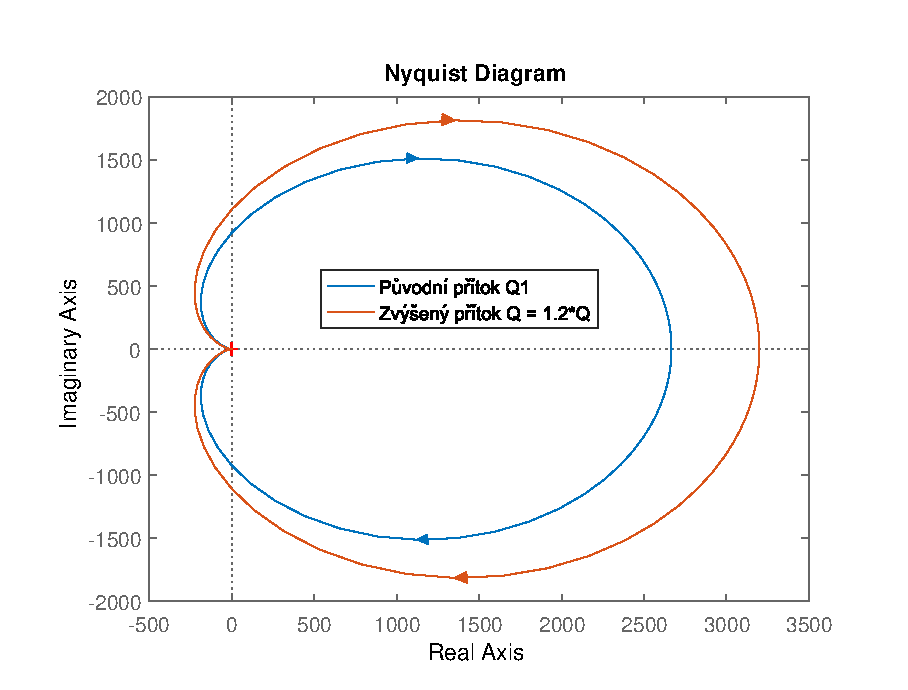
\includegraphics[scale = 1.0]{obrazky/nyquistA.eps}
	\caption{Nyquistova frekvenční charakteristika pro dané přenosy.}
	\label{fig:nyquist-A}
	\end{center}
\end{figure}

\newpage 
Pro získání přenosů pro systém popsaný v kapitole \ref{sec:2B} budeme postupovat stejně a získáme znovu dva přenosy pro pro přítok $ Q_{10} $ ($ P_{1}\left ( s \right )  $) a pro jeho zvýšenou variantu ($ P_{2}\left ( s \right )  $):
\begin{equation}\label{eq:P-B1} 
P_{1}\left ( s \right ) =\frac{20}{s^{2} + 0.25 s + 0.0075}
\end{equation}
\begin{equation}\label{eq:P-B2} 
P_{2}\left ( s \right ) =\frac{24}{s^{2} + 0.3  s + 0.0108},
\end{equation}
jejichž znázornění v komplexní rovině si můžeme prohlédnout na obrázku \ref{fig:nyquist-B}.
\begin{figure}[htbp]
	\begin{center}
	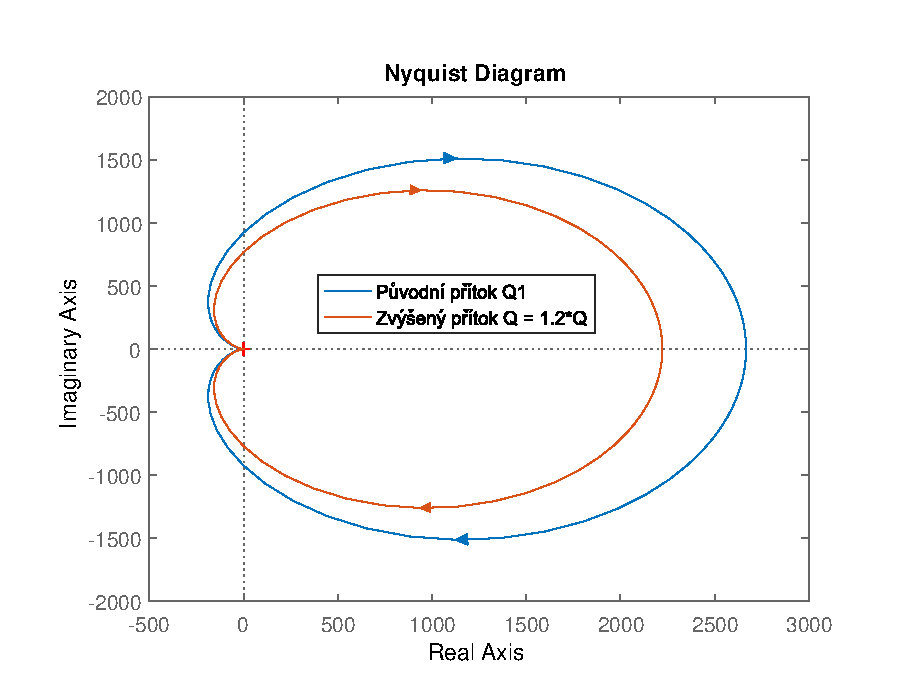
\includegraphics[scale = 1.0]{obrazky/nyquistB.eps}
	\caption{Nyquistova frekvenční charakteristika pro dané přenosy.}
	\label{fig:nyquist-B}
	\end{center}
\end{figure}

\newpage 
\subsubsection{Numerické určení neurčitosti}
Nyní budeme uvažovat, že máme množinový model, ve kterém jsou všechny přenosy $ P $, které vznikly z nominálního přenosu $ P_{0} $ aditivní perturbací:
\begin{equation}\label{eq:Aditivni_neurcitost-zakladni_vztah} 
P = P_{0}+W_{a}\Delta,
\end{equation}
kde $ \left\| \Delta   \right \|_{_{\infty }}< 1 $ a $ W_{a}\left ( s \right ) $ je pevně daná přenosová funkce. Tu můžeme vyjádřit následujícím způsobem:
\begin{equation}\label{eq:Vahova_fce_aditvni} 
W_{a}\left ( s \right ) = P_{0}\left ( s \right )-P\left ( s \right ),
\end{equation}
kde za $ P\left ( s \right ) $ budeme dosazovat přenosy spočtené výše, tedy výsledky \ref{eq:P-A1}, \ref{eq:P-A2}, \ref{eq:P-B1} a \ref{eq:P-B2}. Nejprve se tedy zabývejme přenosy týkající se varianty A, tedy přenosy $ P_{1}\left ( s \right ) $ pro $ Q_{10} $ (viz \ref{eq:P-A1}) a $ P_{1}\left ( s \right ) $ pro $ 1.2\cdot Q_{10} $ (viz \ref{eq:P-A2}) , které jsme spočetli výše. Dále předpokládáme, že pracovní bod se nachází libovolně mezi těmito dvěma pracovními body, lišící se v přítoku $ Q $. Je zřejmé, že nominální model bude vhodné určit pro pracovní bod ležící zhruba uprostřed tohoto intervalu, tedy pro konstantní přítok $ 1.1\cdot Q_{10} $. Při jeho určení budeme postupovat stejně jako během určování $ P_{1}\left ( s \right ) $ a $ P_{2}\left ( s \right ) $. Nominální přenos tedy bude mít tvar:
\begin{equation}\label{eq:P-A0} 
P_{0}\left ( s \right ) =\frac{18.18}{s^{2} + 0.2273 s + 0.006198}.
\end{equation}
Váhovou funkci pro námi zvolenou aditivní neurčitost spočteme ze vztahu \ref{eq:Vahova_fce_aditvni}:   
\begin{equation}\label{eq:Wa-A}
Wa = \frac{1.818 s^{2} + 8.882\cdot 10^{-16}s - 0.0124}{s^{4} + 0.4773 s^{3} + 0.07052 s^{2} + 0.003254 s + 4.649\cdot 10^{-5}}.
\end{equation} 
Zajímavé bude zejména grafické znázornění neurčitosti. To provedeme pro různé kombinace přenosových funkcí, které odpovídají systému za předpokladu různých velikostí konstantních přítoků, přičemž zavedeme omezení: 
\begin{equation}
\label{eq:Q_omezeni} 
Q_{10} \leq Q_{1} \leq 1.2\cdot Q_{10}, 
\end{equation}
z nichž jednomu bude odpovídat námi zvolení nominální model $ P_{0} $. Zobrazení k komplexní rovině je ke shlédnutí na obrázku \ref{fig:neurcitost-A}.
\begin{figure}[htbp]
	\begin{center}
	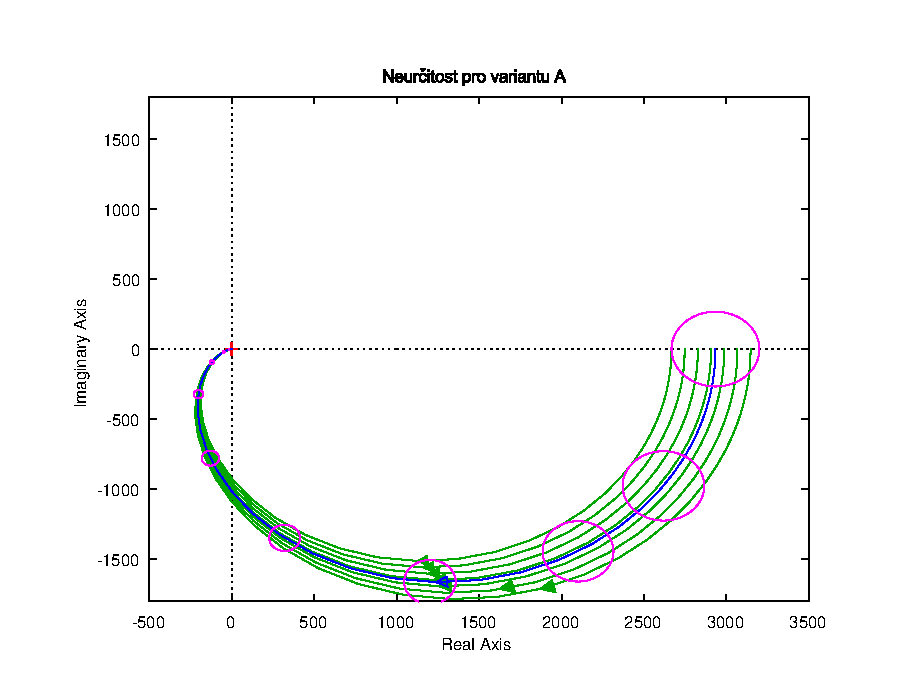
\includegraphics[scale = 1.0]{obrazky/neurcitostA.eps}
	\caption{Grafické znázornění neurčitosti pro variantu A.}
	\label{fig:neurcitost-A}
	\end{center}
\end{figure}

S přenosy $ P_{1}\left ( s \right ) $ a $ P_{2}\left ( s \right ) $ týkajícími se varianty B (viz tvary přenosů \ref{eq:P-B1} a \ref{eq:P-B2}) budeme pracovat stejně. V tomto případě bude mít nominální přenos tvar:
\begin{equation}\label{eq:P-B0} 
P_{0}\left ( s \right ) =\frac{22}{s^{2} + 0.275 s + 0.009075},
\end{equation}
načež dále opět využijeme vztahu \ref{eq:Vahova_fce_aditvni} k určení váhové funkce:
\begin{equation}\label{eq:Wa-B}
Wa = \frac{-2s^{2} + 8.882\cdot 10^{-16}s - 0.0165}{s^{4} + 0.525 s^{3} + 0.08532 s^{2} + 0.004331 s + 6.806\cdot 10^{-5}}.
\end{equation}
Grafické znázornění provedeme rovněž stejně jako v předchozím bodě za respektování omezení \ref{eq:Q_omezeni}. Znázornění je možno vidět na obrázku \ref{fig:neurcitost-B}.
\begin{figure}[htbp]
	\begin{center}
	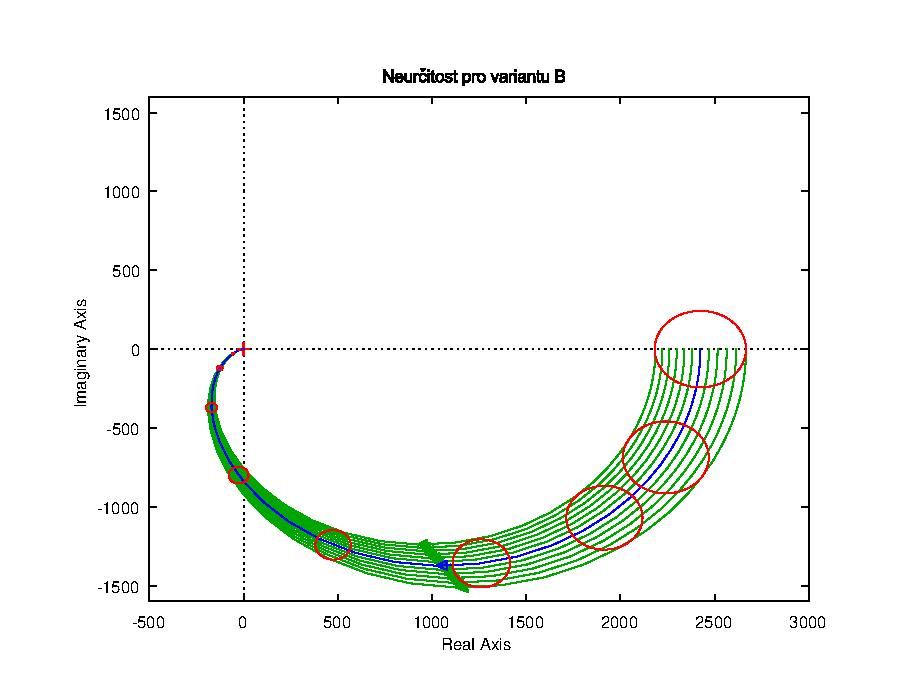
\includegraphics[scale = 1.0]{obrazky/neurcitostB.eps}
	\caption{Grafické znázornění neurčitosti pro variantu B.}
	\label{fig:neurcitost-B}
	\end{center}
\end{figure}

\newpage
Na obrázcích \ref{fig:neurcitost-A} a \ref{fig:neurcitost-B} si všimněme, že je zde vykresleno několik zelených křivek pro přenosové funkce za předpokladu různých, na intervalu \ref{eq:Q_omezeni} vhodně rozmístěných, konstantních přítoků. Modrá křivka představuje náš nominální model $ P_{0} $. V případě aditivní perturbace se velikost neurčitosti rovná $ \left | W_{a} \right | $, která určuje poloměr kružnic, které mají střed na křivce značící nominální přenos. Na obrázcích jich vidíme hned několik, a to pro 10 vhodně zvolených frekvencí $ \omega $, které pokrývají fázové zpoždění $ \left ( 0, 2\pi  \right ) $.

\subsection{Čtvrtý úkol - Porovnání velikostí neurčitostí}
Porovnání neurčitostí pro oba případy provedeme vykreslením příslušných Bodeho frekvenčních charakteristik, kde pozorujeme nepatrné rozdíly, viz obrázek \ref{fig:porovnani_neurcitosti}.
\begin{figure}[htbp]
	\begin{center}
	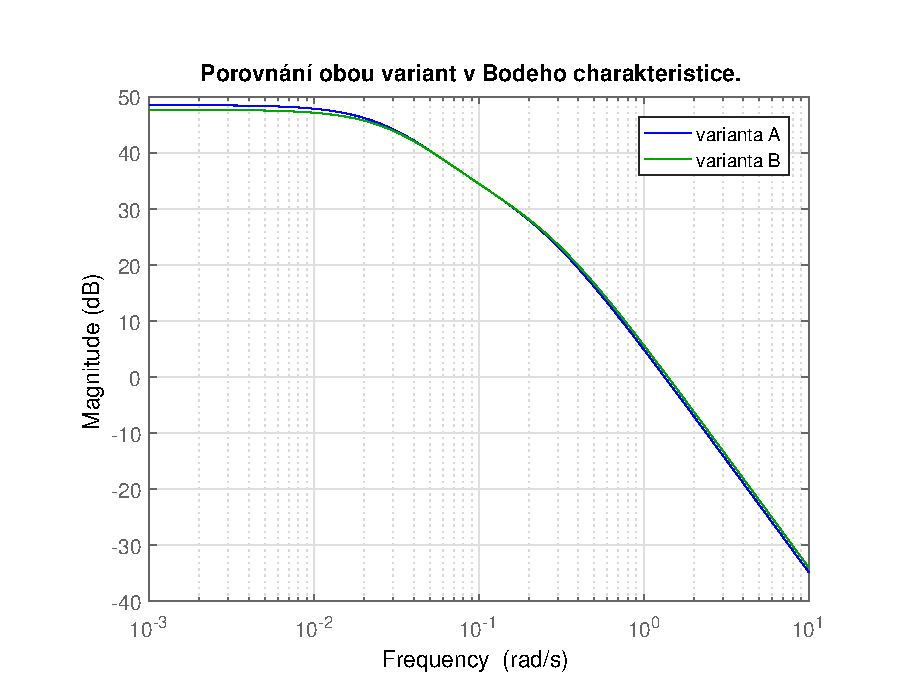
\includegraphics[scale = 1.0]{obrazky/porovnaniNeurcitosti.eps}
	\caption{Porovnání neurčitostí}
	\label{fig:porovnani_neurcitosti}
	\end{center}
\end{figure}


\newpage
\section{Řešení - Návrh regulátoru}
V následující čísti budeme předpokládat, že přítok $ Q_{1}\left ( t \right ) $ již není konstantní, ale je realizován vodním čerpadlem, jehož chování budeme aproximovat systémem prvního řádu s časovou konstantou $ T=0.5s $ a statickým zesílením $ K = Q_{10} $. 
Přenosová funkce od napětí na kotvě stejnosměrného motoru má tedy tvar:
\begin{equation}\label{eq:Prenos_motoru} 
F_{c}\left ( s \right )=\frac{Q_{10}}{1+0.5s}.
\end{equation}
Jelikož se budeme dle zadání snažit pomocí PI regilátoru (viz kapitola \ref{sec:PI}) řídit výšku hladiny $ H_{2} $, vybereme přenos systému z kapitoly \ref{sec:2A}, kde uvažujeme variantu A, tedy měnící se hladiny. Použijeme tudíž (nominální) přenos systému (viz \ref{eq:P-A0}) a se zahrnutím přenosu motoru čerpadla (viz \ref{eq:Prenos_motoru}) získáme přenos soustavy ve tvaru:
\begin{equation}\label{eq:Prenos_soustavy_s_motorem-nominalni} 
P_{S0}\left ( s \right )=F_{c}\left ( s \right )\cdot P_{0}\left ( s \right )=\frac{0.002727}{0.5 s^{3} + 1.114 s^{2} + 0.231 s + 0.0062}.
\end{equation}
Vedle nominálního přenosu budeme použijeme ještě dva další přenosy. Nejvhodnější bude uvažovat právě mezní situace, tedy pro případ minimálního přítoku $ Q_{10} $ a maximálního uvažovaného (zvýšeného) přítoku $ 1.2\cdot Q_{10} $. Přenosy pro tyto varianty jsme spočetli v \ref{eq:P-A1} a \ref{eq:P-A2}. Po dosazení získáme:
\begin{equation}\label{eq:Prenos_soustavy_s_motorem-min} 
P_{S1}\left ( s \right )=F_{c}\left ( s \right )\cdot P_{1}\left ( s \right )=\frac{0.003}{ 0.5 s^3 + 1.125 s^2 + 0.2537 s + 0.0075}
\end{equation}
\begin{equation}\label{eq:Prenos_soustavy_s_motorem-max} 
P_{S2}\left ( s \right )=F_{c}\left ( s \right )\cdot P_{2}\left ( s \right )=\frac{0.002501}{0.5 s^3 + 1.104 s^2 + 0.2109 s + 0.005208}.
\end{equation}

\subsection{První úkol - návrh parametrů PI regulatoru}\label{sec:PI} 
Dále budeme uvažovat, že napětí na kotvě motoru čerpadla je řízeno pomocí PI regulátoru za účelem řídit výšku hladiny $ H_{2} $. Ještě poznamenejme, že  dle podmínek uvedených v zadání můžeme systém považovat za lineární. Přenos PI regulátoru bude mít tvar:
\begin{equation}\label{eq:Prenos_regulatoru} 
C\left ( s \right )=K\cdot \left ( 1+\frac{1}{T_{i}s} \right ).
\end{equation}
Úkolem je navrhnout parametry PI regulátoru tak, aby byly splněny návrhové požadavky pro všechny systémy z modelu neurčitosti pro variantu A, tedy pro měnící se výšky hladin. Tím je myšleno, že požadavky budou platit pro libovolný pracovní bod, který se nachází mezi původním pracovním bodem a pracovním bodem při zvýšením přítoku, tedy pro takový přítok $ Q $, který splňuje podmínku \ref{eq:Q_omezeni}. 

Pro návrh parametrů PI regulátoru jsme využili Matlabovský nástroj PID Tuner. Výsledkem je určení $ K $ a $ T_{i} $:
$$ K = 10 $$ 
$$ T_{i} = 0.1 $$
Regulátor tedy bude mít po dosazení do \ref{eq:Prenos_regulatoru} přenos:
\begin{equation}\label{eq:Vypocteny_prenos_regulatoru} 
C\left ( s \right )=K\cdot \left ( 1+\frac{1}{T_{i}s} \right ) = \frac{10s+0.1}{s}.
\end{equation}
V další části se budeme zabývat návrhovými požadavky.
%\frac{83.25s+10.9023}{s} - ZNF

\newpage
\subsubsection{Vnitřní stabilita uzavřené smyčky}
Pro grafické ověření vnitřní stability poslouží Nyquistovo kritérium. K jeho použití potřebujeme znát přenos otevřené smyčky $ L_{0} $:
\begin{equation}\label{eq:L0} 
L_{0}=CP_{S0}=\frac{ 0.02727 s + 0.0002727}{0.5 s^{4} + 1.114 s^3 + 0.231 s^2 + 0.0062 s}.
\end{equation}
\begin{equation}\label{eq:Lmin} 
L_{1}=CP_{S1}=\frac{0.03 s + 0.0003}{0.5 s^4 + 1.125 s^3 + 0.2537 s^2 + 0.0075 s}.
\end{equation}
\begin{equation}\label{eq:Lmax} 
L_{2}=CP_{S2}=\frac{0.025 s + 0.0002501}{0.5 s^4 + 1.104 s^3 + 0.2109 s^2 + 0.005208 s}.
\end{equation}
Nyní zjistěme počet nestabilních pólů $ P $ a nestabilních nul $ Z $ a definujme:
\begin{equation}\label{eq:N=P-Z} 
N=P-Z.
\end{equation}
Z přenosu zjistíme, že $ P=1 $ a $ Z=0 $, tedy $ N=1 $ pro všechny tři případy. Nyquistovo kritérium stability říká, že křivka $ L_{0}\left ( j\omega \right )  $ musí obkličovat bod $ \left ( -1,0 \right ) $ právě \textit{N}-krát v kladném směru. Vykresleme tedy Nyquistovu křivku pro otevřený systém.

\begin{figure}[htbp]
	\begin{center}
	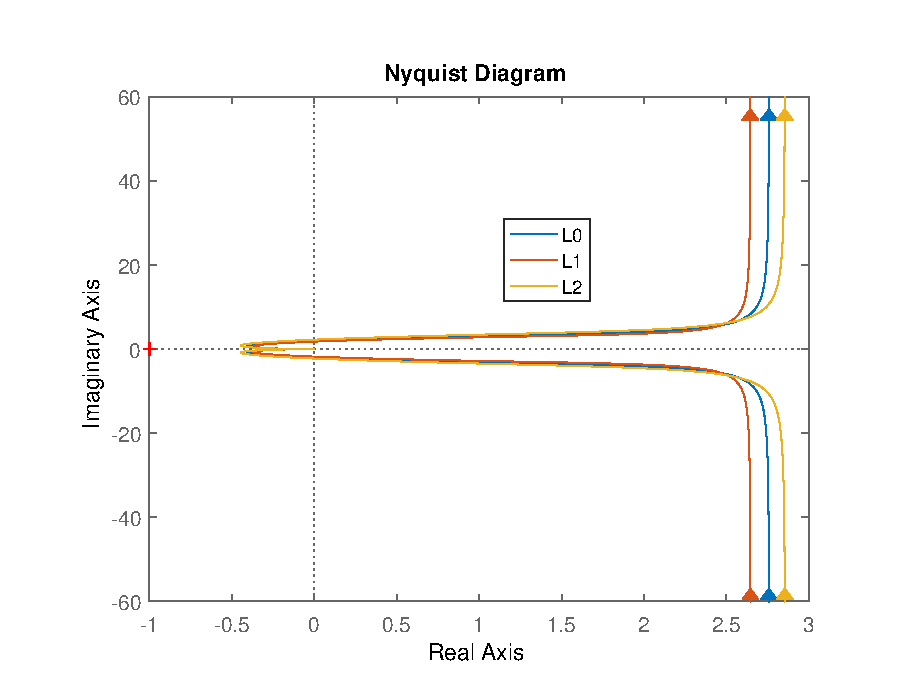
\includegraphics[scale = 1.0]{obrazky/nyquist.eps}
	\caption{Grafická interpretace Nyquistova kritéria stability.}
	\label{fig:Nyquistovo_kriterium_stability}
	\end{center}
\end{figure}

Z Nyquistovy křivky na obrázku \ref{fig:Nyquistovo_kriterium_stability} vidíme, že že křivka $ L_{0}\left ( j\omega \right )  $ obkličuje bod $ \left ( -1,0 \right ) $ právě jednou v kladném směru, což je důkaz splnění Nyquistova kritéria stability.


\newpage 
Analyticky ověříme vnitřní stabilitu pomocí známého faktu, že zpětnovazební systém je vnitřně stabilní právě tehdy, jestliže jeho charakteristický polynom nemá žádné nuly v oblasti $ Re\left ( s \right )\geq 0. $
Charakteristický polynom má tvar:
\begin{equation}
1+L_{0}=1+CP_{S0}=\frac{0.5 s^4 + 1.114 s^3 + 0.231 s^2 + 0.03347 s + 0.0002727}{ 0.5 s^4 + 1.114 s^3 + 0.231 s^2 + 0.0062 s}
\end{equation}
\begin{equation}
1+L_{1}=1+CP_{S1}=\frac{0.5 s^4 + 1.125 s^3 + 0.2537 s^2 + 0.0375 s + 0.0003}{0.5 s^4 + 1.125 s^3 + 0.2537 s^2 + 0.0075 s}
\end{equation}
\begin{equation}
1+L_{2}=1+CP_{S2}=\frac{0.5 s^4 + 1.104 s^3 + 0.2109 s^2 + 0.03021 s + 0.0002501}{0.5 s^4 + 1.104 s^3 + 0.2109 s^2 + 0.005208 s}.
\end{equation}
Jak můžeme pozorovat, charakteristický polynom ani v jednom případě žádné nestabilní nuly neobsahuje. I tato podmínka stability je tedy splněna.

\newpage
\subsubsection{Robustnost ve stabilitě}
Zde budeme pracovat se dvěma důležitými přenosy, a to s citlivostní funkcí:
\begin{equation}
S_{0}=\frac{1}{1+CP_{S0}}
\end{equation}
a s komplementární citlivostní funkcí
\begin{equation}
T_{0}=\frac{CP_{S0}}{1+CP_{S0}}.
\end{equation}
Máme požadavek, aby maximální hodnota amplitudy citlivostní funkce byla omezena:
\begin{equation}\label{eq:Amplituda_citlivostky} 
M_{S}<2.
\end{equation}
Pro určení váhové funkce $ W_{1} $ využijeme podmínku kvality řízení pro nominální přenos $ P_{0} $, kde musí platit:
\begin{equation}
\left \| S_{0} \right \|_{\infty }<2,
\end{equation}
\begin{equation}
\left \| W_{1}S_{0} \right \|_{\infty }<1,
\end{equation}
a tedy $  W_{1} $ nastavíme na $ 0.5 $. Po dosazení zjistíme, že protože:
\begin{equation}
\left \| W_{1}S_{0} \right \|_{\infty }=0.6767<1,
\end{equation}
je podmínka \ref{eq:Amplituda_citlivostky} splněna.
Pro zajímavost můžeme prozkoumat i robustní kvalitu řízení. Pro tu musí platit nutná a postačující podmínka:
\begin{equation}\label{eq:Robustni_kvalita_podminka} 
\left \| \left | W_{1}S_{0} \right |+ \left | W_{2}T_{0} \right |\right \|_{\infty }< 1,
\end{equation}
kde $  W_{1} $ specifikuje kvalitu řízení a $  W_{2} $ specifikuje neurčitost systému. Tu určíme využitím přenosu $  W_{a} $ (viz \ref{eq:Wa-A}) takto:
\begin{equation}\label{eq:Wm=Wa/P0} 
W_{2}=W_{m}=\frac{W_{a}}{P_{0}}=\frac{1.818 s^{4} + 0.4144 s^{3} - 0.001124 s^{2} - 0.002825 s - 7.686e-05}{18.18 s^{4} + 8.678 s^{3} + 1.282 s^{2} + 0.05917 s + 0.0008452},
\end{equation}
kde $ W_{m} $ specifikuje neurčitost systému, pokud bychom uvažovali multiplikativní perturbaci. My ale pracujeme s aditivní neurčitostí danou $ W_{a} $, jejíž znalost využijeme pro výpočet $ W_{m} $ pro náš případ (viz \ref{eq:Wm=Wa/P0}). Po tomto ujasnění již můžeme pracovat se známými vztahy.
Dosazením do \ref{eq:Robustni_kvalita_podminka} získáme:
\begin{equation} 
\left \| \left | W_{1}S_{0} \right |+ \left | W_{2}T_{0} \right |\right \|_{\infty }= 0.7077 <1.
\end{equation}
Nutná a postačující podmínka pro robustní kvalitu řízení je tedy splněna. Nyní ověřme podmínku pro robustní stabilitu, která říká:
\begin{equation} 
\left \| W_{2}T_{0}\right \|_{\infty }<1.
\end{equation}
Po dosazení získáme:
\begin{equation} 
\left \| W_{2}T_{0}\right \|_{\infty }=0.082<1.
\end{equation}
Ověřili jsme si tedy robustnost ve stabilitě pro danou množinu modelů.

\newpage 
\subsubsection{Podmínka útlumu komplementrání citlivostní funkce}
Útlum komplementární citlivostní funkce $ T\left ( j\omega \right ) $ na frekvenci $ \Omega _{a}=10 \left[ rad\cdot s^{-1}   \right ] $, na kterou je omezená dostupná šířka pásma, musí být alespoň $ -10 $ dB. K ověření tohoto požadavku si vykresleme Bodeho frekvenční charakteristiky:
\begin{figure}[htbp]
	\begin{center}
	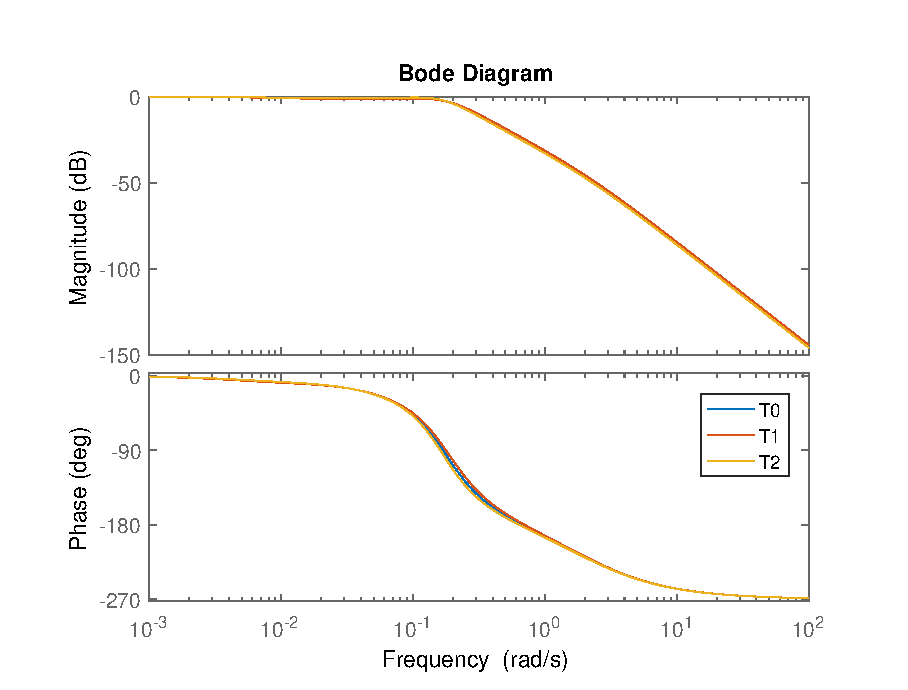
\includegraphics[scale = 1.0]{obrazky/citlivostniFunkce.eps}
	%\caption{Nyquistova frekvenční charakteristika pro dané přenosy.}
	\label{fig:citlivostka}
	\end{center}
\end{figure}

Vyčteme, že útlum na frekvenci $ \Omega _{a} $ je roven pro varianty přenosu 0, 1 a 2: 
-85.4368, -84.6093 a -86.1905 dB, což náš požadavek bohatě splňuje.


\subsubsection{Omezení zesílení energie šumu}
Posledním požadavkem je zajistit, aby energie libovolného šumu měření $ n\left ( t \right ) $ nebyla zesílena více než 1.5 krát. K výpočtu hodnoty tohoto zesílení poslouží $ \left \| H \right \|_{\infty } $ norma komplementární citlivostní funkce:
\begin{equation}
\left \| T_{0} \right \|_{\infty } = 1.0 <1.5.
\end{equation}
I tohoto omezení jsme tedy docílili. Platnost si opět ověřme i pro další přenosy množinového modelu.
\begin{equation}
\left \| T_{1} \right \|_{\infty } = 1.0 <1.5.
\end{equation}
\begin{equation}
\left \| T_{2} \right \|_{\infty } = 1.0 <1.5.
\end{equation}

\newpage 
\subsection{Druhý úkol - kontrola zesílení poruch}\label{sec:2_2} 
V dalším kroku budeme budeme předpokládat, že měření, které provádí senzor hladiny $ H_{2} $, bude zatíženo harmonickým šumem $ n\left ( t \right ) $ o frekvenci 50 Hz. Je známo, že pokud $ n\left ( t \right ) $ je šum měření, je přenos $ n\rightarrow y $ má tvar:
\begin{equation}
-T\left ( j\omega  \right ) = \frac{-C\left ( j\omega  \right )P\left (j\omega  \right )}{1+ C\left ( j\omega  \right )P\left ( j\omega  \right )}.
\end{equation}
Nyní dosazením dané frekvence $ \omega = 2\pi \cdot 50 $ zjistíme, zda je signál zesílen.
$$ \left | -T_{0}\left ( j\omega  \right ) \right | = 1.7618\cdot 10^{-9}$$
$$ \left | -T_{1}\left ( j\omega  \right ) \right | = 1.9380\cdot 10^{-9}$$
$$ \left | -T_{2}\left ( j\omega  \right ) \right | = 1.6153\cdot 10^{-9}.$$
Vidíme tedy, že takovéto šumy měření jsou na výstupu výrazně zeslabeny.
Dále předpokládáme, že i výstup soustavy je zatížen omezenou harmonickou poruchou $ d\left ( t \right ) $ o frekvenci 0.1 Hz. Opět víme, že pokud$ d\left ( t \right ) $ zatěžuje výstup soustavy, je přenos $ d\rightarrow y $ vyjádřen jako:
\begin{equation}
S\left ( j\omega  \right ) = \frac{1}{1+ C\left ( j\omega  \right )P\left ( j\omega  \right )}.
\end{equation}
Opět dosadíme danou frekvenci šumu, tedy $ \omega = 2\pi \cdot 0.1 $, a zkontrolujme zesílení na výstupu.
$$ \left | S_{0}\left ( j\omega  \right ) \right | = 1.0671 $$
$$ \left | S_{1}\left ( j\omega  \right ) \right | = 1.0734 $$
$$ \left | S_{2}\left ( j\omega  \right ) \right | = 1.0617.$$
Zde již naopak pozorujeme mírné zesílení
šumů na výstupu systému.
\subsection{Třetí úkol - určení maximálního kolísání hladiny}
Předpokládejme, že je systém v rovnovážném stavu a regulační odchylka $ e\left ( t \right )=0 $. Na vstup řízené soustavy začíná působit porucha $ d_{i} $ s omezenou energií $ \left \| d_{i} \right \|_{2}<1 $. Cílem bude určit maximální kolísání hladiny $ H_{2} $, ke kterému by mohlo od požadovaného stavu dojít.
Víme, že přenos $ d_{i}\rightarrow y $ bude ve tvaru:
\begin{equation}\label{eq:P/1+CP} 
\frac{P\left (j\omega  \right )}{1+ C\left ( j\omega  \right )P\left ( j\omega  \right )}.
\end{equation}
Dále využijeme znalosti, že pokud velikost vstupu je měřena pomocí $ \left \| H \right \|_{2} $ normy a výstup $ \left \| H \right \|_{\infty }$ normou, bude zesílení systému dáno $ \left \| H \right \|_{2} $ normou přenosu zmíněného přenosu \ref{eq:P/1+CP}. Platí tedy: 
\begin{equation}
\left \| H \right \|_{2}=\sup_{\left \| u \right \|_{2}=1}\frac{\left \| y \right \|_{\infty }}{\left \| u \right \|_{2}}
\end{equation}
Spočtením $ \left \| H \right \|_{2} $ normy znovu pro včechny tři případy získáme:
$$ \left \| \frac{P_{0}\left (j\omega  \right )}{1+ C\left ( j\omega  \right )P\left ( j\omega  \right )} \right\|_{2} = 0.0232 $$
$$ \left \| \frac{P_{1}\left (j\omega  \right )}{1+ C\left ( j\omega  \right )P_{1}\left ( j\omega  \right )} \right \|_{2} = 0.0229 $$
$$ \left \| \frac{P_{2}\left (j\omega  \right )}{1+ C\left ( j\omega  \right )P_{2}\left ( j\omega  \right )} \right \|_{2} = 0.0235$$


\newpage 
\subsection{Čtvrtý úkol - určení nejvíce zesílených signálů}
Nakonec určíme signály $ d\left ( t \right ) $ a $ n\left ( t \right )  $, jejichž $ \left \| h \right \|_{\infty } $ norma je omezená na:
\begin{equation}
\left \| d\left ( t \right ) \right \|_{\infty }<1,
\end{equation}
\begin{equation}
\left \| n\left ( t \right ) \right \|_{\infty }<1.
\end{equation}
Tyto signálu jsou zpětnovazební smyčkou nejvíce zesíleny buďto ve smyslu maximální hodnoty signálu, nebo ve smyslu energie signálu. Ke zjištění, na jakých frekvencích jsou tyto signály zesíleny nejvíce, nám pomůže vykreslení Bodeho frekvenčních charakteristik záporné komplementární citlivostní funkce $ -T\left ( j\omega  \right ) $ a citlivostní funkce $ S\left ( j\omega  \right ) $, určených v kapitole \ref{sec:2_2} pro nominální systém a tyto hodnoty z nich vyčíst.
\begin{figure}[htbp]
	\begin{center}
	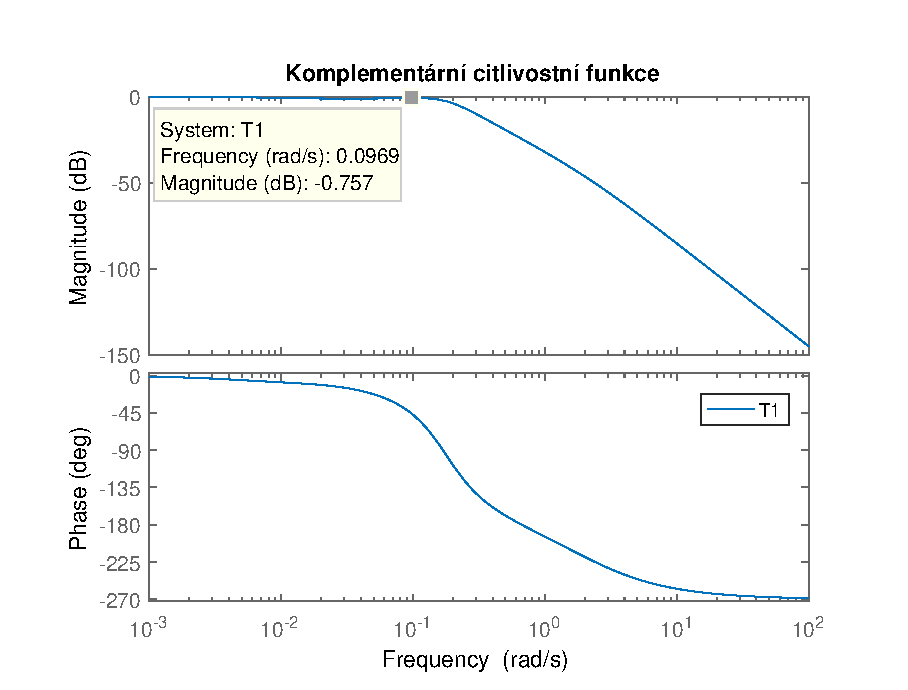
\includegraphics[scale = 1.0]{obrazky/komplementarniFunkceCtyrka.eps}
	\caption{Bodeho frekvenční charakteristika pro $ -T\left ( j\omega  \right ) $.}
	\label{fig:4_-T}
	\end{center}
\end{figure}

\begin{figure}[htbp]
	\begin{center}
	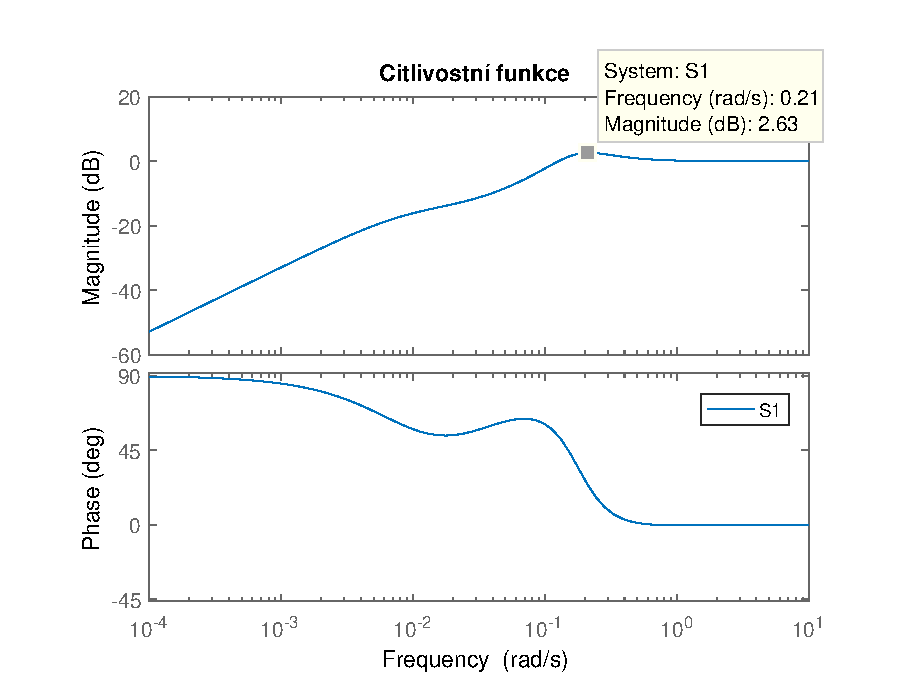
\includegraphics[scale = 1.0]{obrazky/citlivostniFunkceCtyrka.eps}
	\caption{Bodeho frekvenční charakteristika pro $ S\left ( j\omega  \right ) $.}
	\label{fig:4_S}
	\end{center}
\end{figure}

Z každého Bodeho diagramu (obrázky \ref{fig:4_-T} a \ref{fig:4_S}) odečteme jednu frekvenci, tedy v našem případě:
\begin{equation} \label{eq:Omega_n}
\Omega _{n}= 0.097\; \textup{rad}\cdot\textup{s}^{-1}
\end{equation}
\begin{equation}\label{eq:Omega_d} 
\Omega _{d}= 0.21\; \textup{rad}\cdot\textup{s}^{-1}.
\end{equation}


\newpage 
\subsubsection{Ve smyslu maximální hodnoty signálu}
Největší zesílení daných externích signálů budeme pozorovat v případě působení periodických signálů o námi určených frekvencích $ \Omega _{n} $ a $ \Omega _{d}$ (viz \ref{eq:Omega_n} a \ref{eq:Omega_d}). Pokud zesílení uvažujeme ve smyslu maximální hodnoty, bude tento periodický signál představovat obdélníkový signál s příslušnou frekvencí, tedy:
\begin{equation}
u\left ( t-\tau  \right ) \overset{\mathrm{}\triangle}{=}\textup{sgn}\left ( h\left ( \tau  \right ) \right ),
\end{equation}
což lze vyčíst ze známých tabulek stejně tak jako tvar určující zesílení $\left \| h \right \|_{1}$, což je jednotková norma impulsní funkce přenosu $ T\left ( j\omega  \right ) $ pro poruchu měření $ n\left ( t \right ) $ a přenosu $ S\left ( j\omega  \right ) $ pro poruchu na výstupu systému $ d\left ( t \right ) $, přičemž platí:
\begin{equation}
\left |  y\left (t  \right )\right |\leq \left \| h \right \|_{1}\left \| u \right \|_{\infty }.
\end{equation}
Výsledkem je:
$$ \left \| h_{T_{0}} \right \|_{1} = 2.4253 ,$$
$$ \left \| h_{S_{0}} \right \|_{1} = 2.4253 .$$



%\begin{figure}[htbp]
%	\begin{center}
%	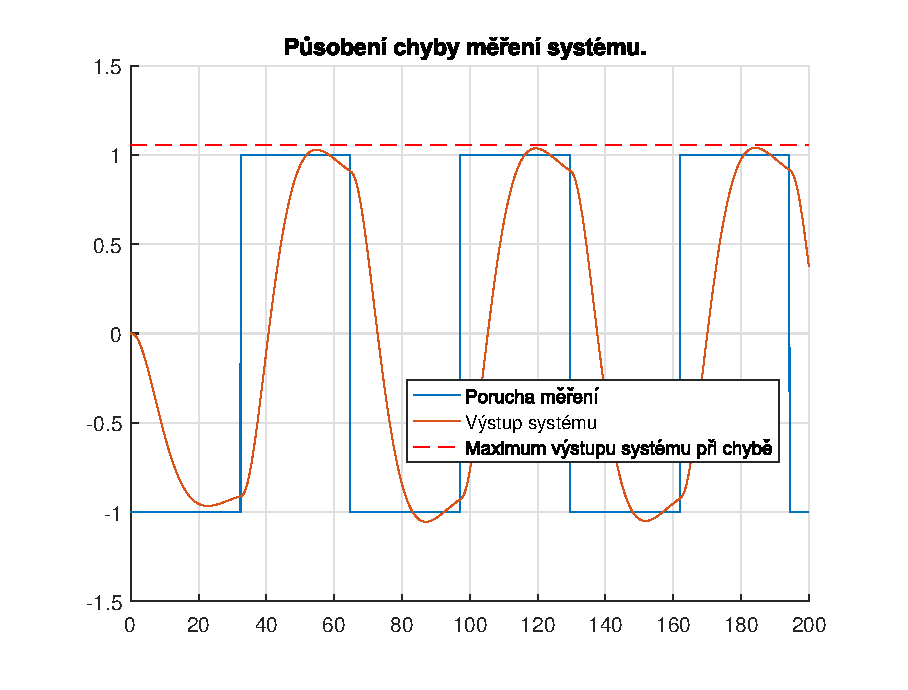
\includegraphics[scale = 1.0]{obrazky/nT2.eps}
%	\caption{Odezva systému při působení obdélníkové poruchy měření $ n\left ( t \right ) $.}
%	\label{fig:4_maxval-n}
%	\end{center}
%\end{figure}

%\begin{figure}[htbp]
%	\begin{center}
%	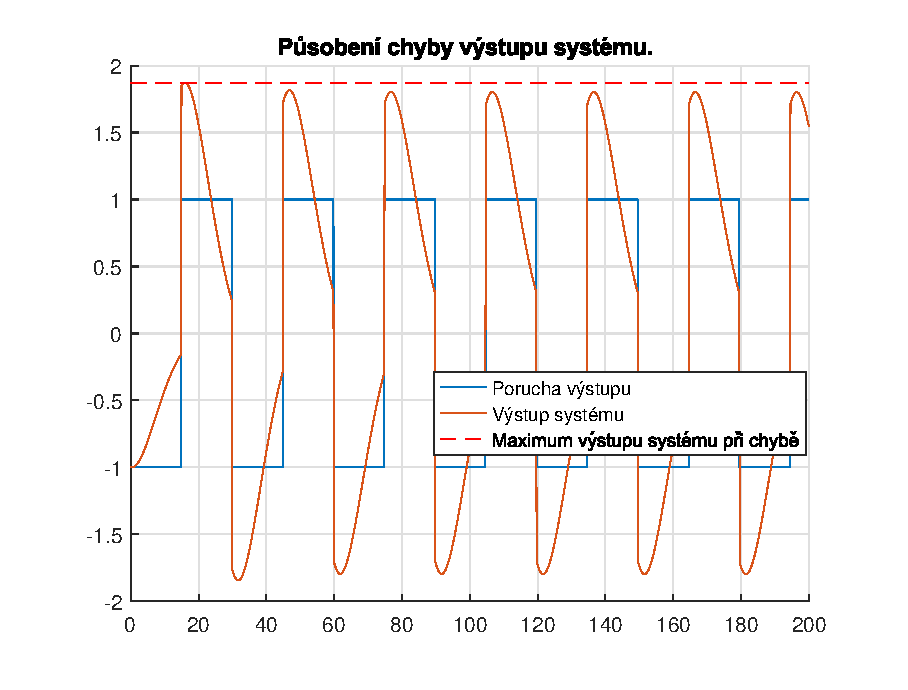
\includegraphics[scale = 1.0]{obrazky/dS2.eps}
%	\caption{Odezva systému při působení obdélníkové poruchy $ d\left ( t \right ) $ na výstup soustavy.}
%	\label{fig:4_maxval-d}
%	\end{center}
%\end{figure}



\newpage 
\subsubsection{Ve smyslu energie signálu}
Pokud zesílení uvažujeme ve smyslu energie, bude působící periodický signál představovat sinusovku s příslušnou frekvencí. Amplitudu zvolíme jednotkovou.
\begin{figure}[htbp]
	\begin{center}
	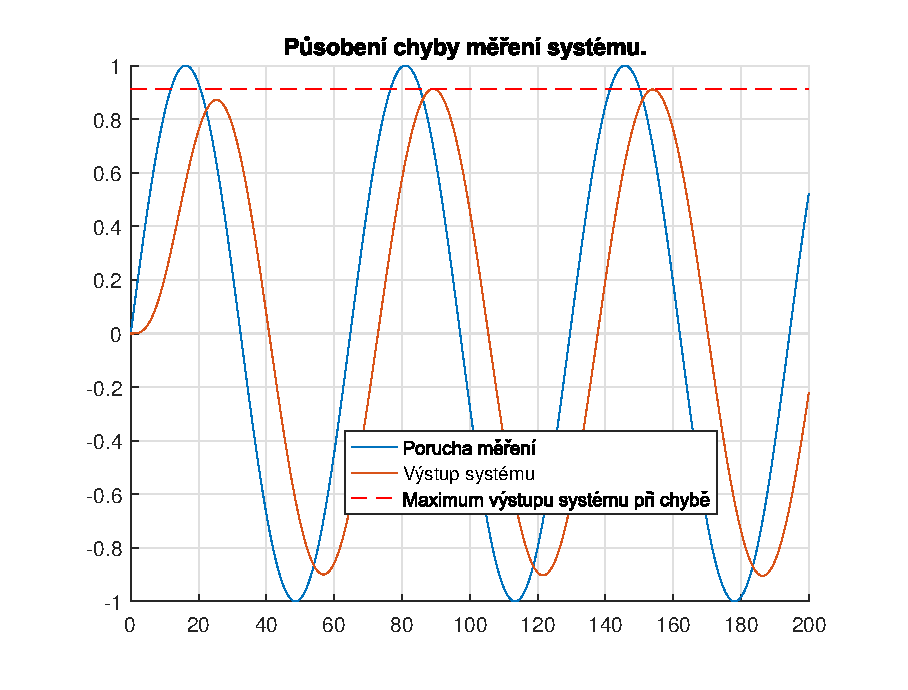
\includegraphics[scale = 1.0]{obrazky/nT.eps}
	\caption{Odezva systému při působení sinusové poruchy měření $ n\left ( t \right ) $.}
	\label{fig:4_energie-n}
	\end{center}
\end{figure}

\begin{figure}[htbp]
	\begin{center}
	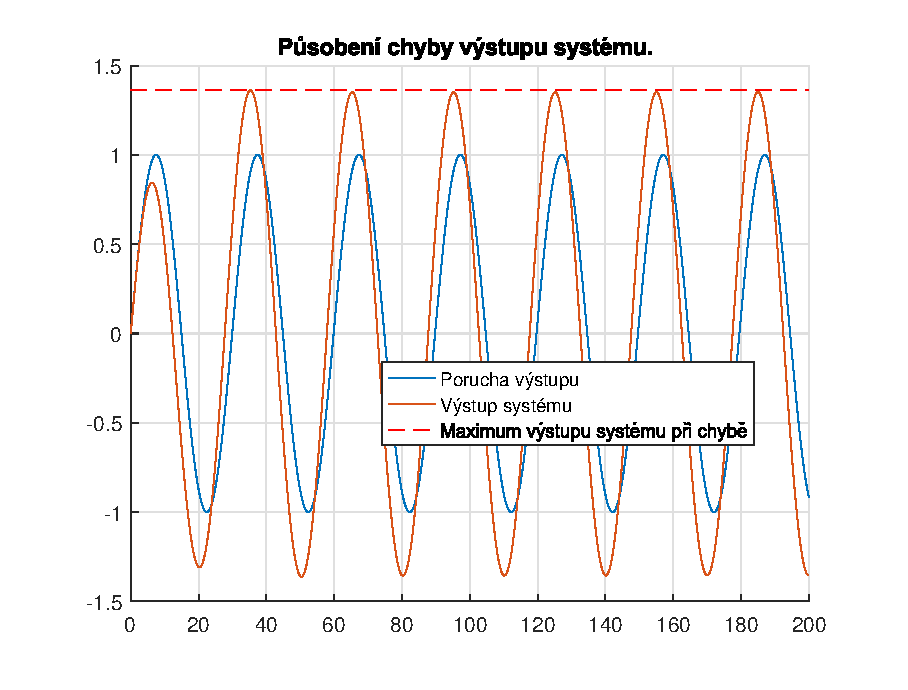
\includegraphics[scale = 1.0]{obrazky/dS.eps}
	\caption{Odezva systému při působení sinusového poruchy $ d\left ( t \right ) $ na výstup soustavy.}
	\label{fig:4_energie-d}
	\end{center}
\end{figure}

Z obrázků \ref{fig:4_-T} a \ref{fig:4_S} můžeme vyčíst, že maximální zesílení na výstupu za předpokladu působení poruchy měření $ n\left ( t \right ) $ je -0.758 dB a v případě působení poruchy $ d\left ( t \right ) $ na výstup soustavy činí 2.63 dB. Z grafů na obrázcích \ref{fig:4_energie-n} a \ref{fig:4_energie-d} snadno vyčteme hodnotu maximálního zesílení. Pokud převedeme tyto hodnoty do jednotek dB, získáme pro poruchu měření $ n\left ( t \right ) $ zesílení -0.7855 dB a pro poruchu na výstupu soustavy $ d\left ( t \right ) $ zesílení  2.6851 dB. Všimněme si, že tyto hodnoty téměř přesně odpovídají těm, které jsme odečetli z Bodeho frekvenční charakteristiky.



\newpage 
\section{Závěr}
Prví polovina práce se zabývá určením linearizovaného stavového modelu v různých pracovních bodech, lišících se ve velikosti přítoku. Rovněž jsme uvažovali dvě varianty, a to jak měnící se výšky hladin, tak i konstantní hladiny za měnícího se nastavení ventilů. Pro všechny případy jsme dále určili přenosové funkce a dále jsme se zabývali neurčitostí. Jako model neurčitosti jsme volili aditivní perturbaci, přičemž jsme zajistili, aby neurčitost byla minimální, ale přesto pokrývala skutečnou neurčitost systému. Neurčitosti pro obě varianty jsme následně porovnali.

V druhé polovině práce jsme řešili návrh regulátoru. Navíc se nám systém ještě rozrostl o přenos motoru čerpadla, který realizoval přítok. Pro jednoduchost jsme jej realizovali pomocí aproximace systémem prvního řádu. Hlavním úkolem bylo navrhnout parametry PI regulátoru, tak aby byla splněna řada uvedených kritérií. Vedle těch základních, jako je například vnitřní stabilita uzavřené smyčky, jsme, jelikož pracujeme s neurčitostí, řešili rovněž robustnost ve stabilitě. K ověřování některých kritérií jsme používali také grafické metody. V dalším bodě jsme uvažovali zatížení senzoru hladiny a výstupu soustavy harmonickými šumy a zjišťovali jsme, zda jsou tyto signály na výstupu uzavřené smyčky zesíleny, nebo tlumeny. Dále jsme určili maximální hodnotu kolísání měřené hladiny za přítomnosti poruchy působící na vstup soustavy. V posledním bodě jsme zkoumali signály jako poruchy působící na senzor měření a na výstup soustavy a hledali jsme, kde jsou zpětnovazební smyčkou nejvíce zesíleny, a to ve smyslu maximální hodnoty signálu, kde jsme je uvažovali jako obdélníkový periodický signál, a ve smyslu energie signálu, kde jsme je interpretovali jako sinusový signál.


\end{document}      
